



%\subsection{Liquid velocity fluctuation}





Objectives : 
\begin{itemize}
    \item Present the decomposition of the fluid reynolds stress according to isotropic and deviatoric part.
    \item Show the relation between the flowlines graphs and the actual values of the fluid velocity fluctuation.
    \item Compare our case with the fits of  \citet{almeras2019fluctuations} 
    \item Compare the fluctuation with theoretical dev \citet{lance1991turbulence,zhang1994ensemble}. 
    \item Find out that the potential flow solution 
    \item Conclusion : " In low inertia regime $B_{xx} = - 0.2$ and $B_{yy} = 0.4$ for all simulations, find out why" (This is also true for the theoretical solution\citep{lance1991turbulence} this is thus due to the form of teh wake)
\end{itemize}



%We decompose both Reynolds stresses into an isotropic part and deviatoric part such that, 
%\begin{align}
%    \bm{\sigma}^{\text{Re}}_p &=  \rho_d \phi_d K^*_p(\textbf{u}_p - \textbf{u}_c)\cdot (\textbf{u}_p - \textbf{u}_c) 
%    \left(
%        \textbf{I}
%        +\textbf{B}_p 
%    \right)\\
%    \bm{\sigma}^{\text{Re}}_c &=  \rho_c \phi_d K_c^*(\textbf{u}_p - \textbf{u}_c)\cdot (\textbf{u}_p - \textbf{u}_c) 
%    \left(
%        \textbf{I}
%        +\textbf{B}_c
%    \right)
%\end{align}
%where the $K^*$ is the dimensionless pseudo-turbulent  kinetic energy, $\textbf{I}$ a unit tensor and $\textbf{B}$ a tensor accounting for the deviation of the Reynolds stress left to determine. 



In the following subsection we present our numerical results for $K^*$ and $\textbf{B}$ for the dispersed and continuous phase. 
\tb{In this section the results are presenetd in terms of Ga because it is easier to show the tendency}




\subsection{Continuous phase}
\todo{try \citet{almeras2021statistics} fits}
\todo{also check \citet{almeras2019fluctuations} results}
\tb{might be good to plot the velocity field to examine where does the fluctuation arise (pseudo-turbe or turbe)}
Look at \citep{wang2021numerical} and Mahra.. 2015 



In this section we analyze the velocity fluctuation within the suspension for both phases. 
In the Stokes regime, due to the slow decay of the velocity perturbation, the liquid velocity fluctuation in very dilute flow tends to infinity (whether the particle are drops bubbles or solids ) \citep{luke1965}. However in experiments (ham et homsy) et Guazelli no such divergence was observed. Different explanations have been proposed in the litterature (see Guazeeli \& Hinch).

IN the opposite regime of potential flow

Alternatively we can use the decomposition,
\begin{align}
    \phi_c\bm{\sigma}^{\text{Re}}_c &=  \rho_c \phi_d 
    \left[
        B_1\textbf{I}(\textbf{u}_p - \textbf{u}_c)\cdot (\textbf{u}_p - \textbf{u}_c) 
        +B_2 (\textbf{u}_p - \textbf{u}_c) (\textbf{u}_p - \textbf{u}_c) 
    \right]\\
\end{align}
for which $B_1$ and $B_2$ are scalar coefficient. 
This decomposition has the advantage that in the potential flow limit theoretical solution are known such that  $B_1 = -0.15$ and  $B_2 = 0.05$ \citet{zhang1994averaged,wang2021numerical}. 
Lastly, \citet{lance1991turbulence} give also a theoretical solution for $\bm{\sigma}^{Re}_c$ based on the potential flow solution around a spherical particle in translation. 




The fluid averaged kinetic energy can be easily scaled on the numerical results shown \ref{fig:Tf_Bf}(left).
It is shown that for $\lambda= 1$ we observe non monotonic behavior while at $\lambda= 10$ it is decreasing.
Except for the cases $\phi = 0.01$ where we cannot be sure if it is due to statistical error or real physics. 
\begin{figure}[h!]
    \centering
    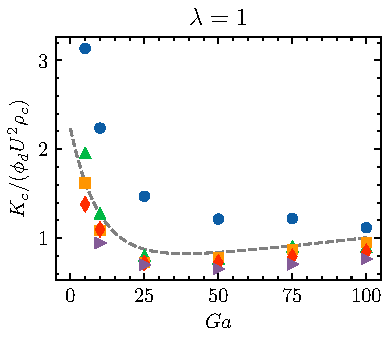
\includegraphics[height=0.3\textwidth]{image/HOMOGENEOUS/fCA/Tf_l_1.pdf}
    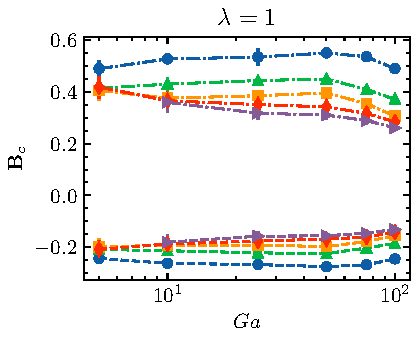
\includegraphics[height=0.3\textwidth]{image/HOMOGENEOUS/fCA/Bf_l_1.pdf}

    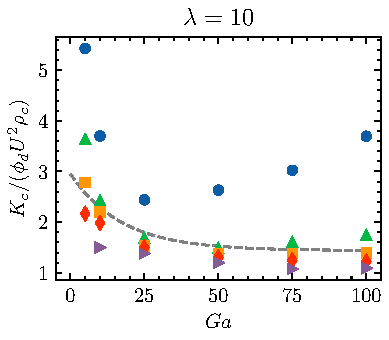
\includegraphics[height=0.3\textwidth]{image/HOMOGENEOUS/fCA/Tf_l_10.pdf}
    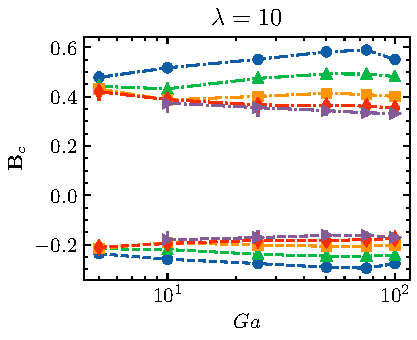
\includegraphics[height=0.3\textwidth]{image/HOMOGENEOUS/fCA/Bf_l_10.pdf}
    \caption{(left) Dimensionless turbulent kinetic energy in terms of the \textit{Galileo} number for different $\phi$. (dots) Numerical simulations, (dashed line) empirical formula \ref{eq:Tf_scaling}.
    The symbols correspond to different volume fraction ($\bullet$) $\phi = 1\%$, ($\blacktriangle$) $\phi = 5\%$, ($\blacksquare$) $\phi = 10\%$, ($\blacklozenge$) $\phi = 15\%$ and ($\blacktriangleright$) $\phi = 20\%$.
    (right) deviatoric part of the Reynolds stress, ($- \cdot -$)  vertical components, $B_{yy}$, ($- -$)  horizontal components, $B_{xx} = B_{zz}$.}
    \label{fig:Tf_Bf}
\end{figure}
\subsection{Dispersed phase}

\tb{Maybe include velocity fluctuation and compare to : Lingxin2021 }

\tb{Include Gaussian distribution of bubbles !!! ! ! ! }

Now let's focus on the particular averaged Reynolds stress tensor.
\ref{fig:Talpha_Balpha} shows that the granular temperature behavior is quite similar from the continuous averaged turbulent kinetic energy.
\begin{figure}[h!]
    \centering
    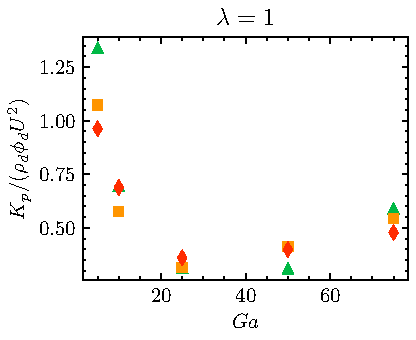
\includegraphics[height=0.3\textwidth]{image/HOMOGENEOUS/fPA/Talpha_l_1.pdf}
    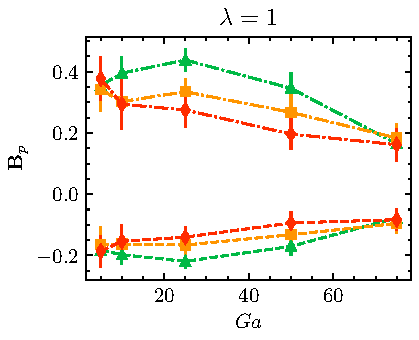
\includegraphics[height=0.3\textwidth]{image/HOMOGENEOUS/fPA/Balpha_l_1.pdf}

    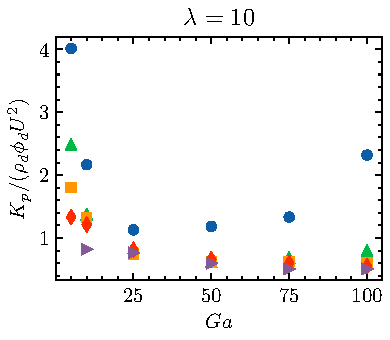
\includegraphics[height=0.3\textwidth]{image/HOMOGENEOUS/fPA/Talpha_l_10.pdf}
    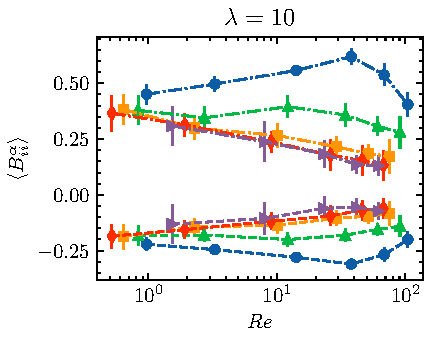
\includegraphics[height=0.3\textwidth]{image/HOMOGENEOUS/fPA/Balpha_l_10.pdf}
    \caption{(left) Dimensionless turbulent kinetic energy $K_p$ in terms of the \textit{Galileo} number for different $\phi$. 
    The symbols correspond to different volume fraction ($\bullet$) $\phi = 1\%$, ($\blacktriangle$) $\phi = 5\%$, ($\blacksquare$) $\phi = 10\%$, ($\blacklozenge$) $\phi = 15\%$ and ($\blacktriangleright$) $\phi = 20\%$.
    (right) deviatoric part of the Reynolds stress, ($- \cdot -$)  vertical components, $B_{yy}$, ($- -$)  horizontal components, $B_{xx} = B_{zz}$.}
    \label{fig:Talpha_Balpha}
\end{figure}
